\section{Constructing King models}
The King model has the distribution function described by the dimensionless potential
\begin{equation}
    f\propto e^W -1
\end{equation}
where 
\begin{equation}
    W(r)\equiv\frac{V(r_t)-V(r)}{\sigma^2}
\end{equation}

Recall that the profile shape only depends on $W_0 \equiv W(0)$ so that the given the
profile, the overall linear size and mass of the profile can be scaled as
desired to any set of units.

\subsection{}
% Note that Poisson’s equation is a second order ordinary differential
% equation just like Newton’s equations and therefore can be written as two coupled first order differential equations. Rewrite the
% Poisson equation as a system of first order ODEs with “physical
% boundary conditions” (that is: $V(0) = $ constant, $dV(0)/dr = 0$) in
% spherical coordinates.
We can solve the King Model by noting that Poisson's equation given by
\begin{equation}
    \nabla^2\psi=-4\pi G\rho.
\end{equation}
can be written into a system of of two first order differential equations in spherical coordinates by first using the chain rule to expand the left term,
\begin{align*}
    \frac{1}{r^2}\frac{d}{dr}\left(r^2\frac{d\psi}{dr}\right)=-4\pi G \rho\\
    \frac{1}{r^2}\left(r^2\frac{d^2\psi}{dr^2}+\frac{d}{dr}(r^2)\frac{d\psi}{dr}\right)=-4\pi G\rho\\
    \frac{d^2\psi}{dr^2}+\frac{1}{r^2}2r\frac{d\psi}{dr}=-4\pi G\rho\\
    \frac{d^2\psi}{dr^2}+\frac{2}{r}\frac{d\psi}{dr}=-4\pi G\rho,\\
\end{align*}

and then we can substitute $y=d\psi/dr$ and rearrange it into
\begin{align*}
    \frac{dy}{dr}+\frac{2y}{r}=-4\pi G\rho\\
    \frac{dy}{dr}=-4\pi G\rho-\frac{2y}{r}.
\end{align*}

So our two differential equations are
\begin{align}
    y&=\frac{d\psi}{dr}
    \label{eq:vpoisson}\\
    \frac{dy}{dr}&=-4\pi G\rho-\frac{2y}{r}
    \label{eq:apoisson}
\end{align}
where $\rho=\rho_K(\psi)$, the king density,
\begin{equation}
    \begin{split}
        \rho_K(\psi)=\rho_1\left[ e^{W}erf(\sqrt{W})-\sqrt{\frac{4W}{\pi}}\left(1+\frac{2W}{3}\right)\right],
    \end{split}
\end{equation}
$W=\psi/\sigma^2$ and $\rho_1=$constant.


\subsection{}

% Integrate (numerically) Poisson’s equation for the King model. By
% adjusting $W_o\equiv W(0)$, one gets models with different concentration; you can check against the table below.
% Plot up the density and the potential just to see what they look like.
% You will use these later on to generate initial conditions for a simulation.
% Check your procedure by computing the values in each of the four columns.
% The core radius of the King model is defined as
% \begin{equation}
%     r_c=\sqrt{9\sigma^2/4\pi G \rho_0}.
% \end{equation}
% In these units, the second column describes the total energy of the King model, the third column describes the concentration, c, the fourth is the the central density in units of
% the mean density and the fifth is the mean square particle radius in
% units of the tidal radius.

Once we have our two first order differential equations (\ref{eq:vpoisson} and \ref{eq:apoisson}), we can use our 4th order Runge-Kutta to integrate them numerically. The initial conditions are $\Psi(0) = W_0\sigma^2 = $ constant and $d\Psi(0)/dr = 0$ where $W_0$ is the dimensionless potential and is shown in the first column of table \ref{tab:KingModel}. 

\begin{figure}
    \centering
    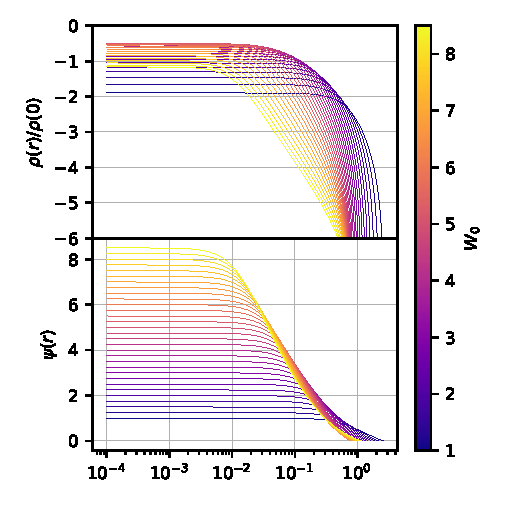
\includegraphics{CodeAndFigures/KingModelPlots.pdf}
    \caption{Plot of the density and potential using the King Model and the initial conditions shown in Table \ref{tab:KingModel}.}
    \label{fig:KingDensityPotential}
\end{figure}

Figure \ref{fig:KingDensityPotential} shows the density and the potential for each case of $W_0$. Note that both start being constant until a value $\log(r)$ where they start getting smaller. 

The second column is the total energy,
\begin{equation}
    E_T=\pi\int\rho\Phi r^2
    \label{eq:TotalEnergy}
\end{equation}
where 
\begin{equation}
    \phi(r) = \phi(r_t)-\Psi(r)
    \label{eq: Potential}
\end{equation}

The third column is the concentration,
\begin{equation}
    c = \log_10(\frac{r_t}{r_c}
\end{equation}
where
\begin{equation}
    r_c=\sqrt{9\sigma^2/4\pi G \rho_0}.
\end{equation}

The fourth column is the central density in units of the mean density given by
\begin{equation}
    \rho_c = \rho(0)/(3M/(4\pi r_t^3)).
\end{equation}

The fifth column is the mean square particle radius given by
\begin{equation}
\langle r^2 \rangle = \frac{\int\rho(\Psi)r^4}{r_t^2 \int\rho(\Psi)r^2}
\end{equation}
where $r_t$ is the last value of r.

\begin{table*}
    \centering
    \begin{tabular}{rrrrr}
\toprule
   $W_0$ &  $E_t/(GM^2/r_t)$ &  $\log_{10}(r_t/r_c)$ &  $\rho(0)/(3M/(4\pi r_t^3))$ &  $<r^2>/r_t^2$ \\
\midrule
1.00e+00 &         -6.41e-01 &              2.95e-01 &                     3.21e+01 &       1.50e-01 \\
1.25e+00 &         -6.54e-01 &              3.57e-01 &                     3.52e+01 &       1.46e-01 \\
1.50e+00 &         -6.68e-01 &              4.11e-01 &                     3.89e+01 &       1.41e-01 \\
1.75e+00 &         -6.83e-01 &              4.59e-01 &                     4.33e+01 &       1.36e-01 \\
2.00e+00 &         -6.99e-01 &              5.05e-01 &                     4.86e+01 &       1.31e-01 \\
2.25e+00 &         -7.17e-01 &              5.48e-01 &                     5.49e+01 &       1.26e-01 \\
2.50e+00 &         -7.37e-01 &              5.90e-01 &                     6.26e+01 &       1.21e-01 \\
2.75e+00 &         -7.59e-01 &              6.31e-01 &                     7.21e+01 &       1.16e-01 \\
3.00e+00 &         -7.83e-01 &              6.72e-01 &                     8.38e+01 &       1.11e-01 \\
3.25e+00 &         -8.09e-01 &              7.13e-01 &                     9.82e+01 &       1.06e-01 \\
3.50e+00 &         -8.38e-01 &              7.54e-01 &                     1.17e+02 &       1.01e-01 \\
3.75e+00 &         -8.69e-01 &              7.96e-01 &                     1.40e+02 &       9.55e-02 \\
4.00e+00 &         -9.05e-01 &              8.40e-01 &                     1.71e+02 &       9.04e-02 \\
4.25e+00 &         -9.44e-01 &              8.85e-01 &                     2.11e+02 &       8.55e-02 \\
4.50e+00 &         -9.88e-01 &              9.31e-01 &                     2.64e+02 &       8.06e-02 \\
4.75e+00 &         -1.04e+00 &              9.79e-01 &                     3.35e+02 &       7.61e-02 \\
5.00e+00 &         -1.09e+00 &              1.03e+00 &                     4.33e+02 &       7.17e-02 \\
5.25e+00 &         -1.15e+00 &              1.08e+00 &                     5.70e+02 &       6.74e-02 \\
5.50e+00 &         -1.21e+00 &              1.14e+00 &                     7.60e+02 &       6.37e-02 \\
5.75e+00 &         -1.29e+00 &              1.19e+00 &                     1.04e+03 &       6.00e-02 \\
6.00e+00 &         -1.37e+00 &              1.25e+00 &                     1.44e+03 &       5.68e-02 \\
6.25e+00 &         -1.45e+00 &              1.32e+00 &                     2.04e+03 &       5.38e-02 \\
6.50e+00 &         -1.55e+00 &              1.39e+00 &                     2.94e+03 &       5.15e-02 \\
6.75e+00 &         -1.64e+00 &              1.46e+00 &                     4.32e+03 &       4.94e-02 \\
7.00e+00 &         -1.75e+00 &              1.53e+00 &                     6.45e+03 &       4.78e-02 \\
7.25e+00 &         -1.85e+00 &              1.60e+00 &                     9.72e+03 &       4.68e-02 \\
7.50e+00 &         -1.94e+00 &              1.68e+00 &                     1.47e+04 &       4.63e-02 \\
7.75e+00 &         -2.02e+00 &              1.76e+00 &                     2.23e+04 &       4.63e-02 \\
8.00e+00 &         -2.09e+00 &              1.83e+00 &                     3.35e+04 &       4.69e-02 \\
8.25e+00 &         -2.12e+00 &              1.91e+00 &                     4.96e+04 &       4.78e-02 \\
8.50e+00 &         -2.14e+00 &              1.98e+00 &                     7.17e+04 &       4.92e-02 \\
\bottomrule
\end{tabular}

    \caption{Table showing from left to right, $W_0$, total energy, concentration, central density, and the mean square particle radius.}
    \label{tab:KingModel}
\end{table*}